\documentclass[12pt,a4paper]{article}
\usepackage{amsmath}
\usepackage{amsfonts}
\usepackage{amssymb}
\usepackage[utf8]{inputenc}
\usepackage[T1,T2A]{fontenc}
\usepackage[english, russian]{babel}
\usepackage{graphicx}
\usepackage[left=2cm,right=2cm,top=2cm,bottom=2cm]{geometry}
\usepackage{calc}
\usepackage{wrapfig}
\usepackage{setspace}
\usepackage{indentfirst}
\usepackage{subfigure}


\title{
Отчет о выполнении лабораторной работы 2.1.4 \\
Определение теплоемкости твердых тел
}

\author{Фокин Алексей, 922 группа}

\begin{document}
\maketitle

	\textbf{Цель работы:} измерение количества подведенного тепла и вызванного им нагрева твердого тела; определение теплоемкости по экстраполяции отношения $\Delta Q / \Delta T$ к нулевым потерям тепла.
	
	\textbf{В работе используются:} калориметр с нагревателем и термометром сопротивления; амперметр; вольтметр; мост постоянного тока; источник питания 36 В.

\section{Теоретическая справка}

В данной работе теплоемкость определяется по формуле
\begin{equation}
	C = \frac{\Delta Q}{\Delta T},
	\label{eq:dQdT}
\end{equation}

где $\Delta Q$ -- количество тепла, подведенного к телу, и $\Delta T$ -- изменение температуры тела, произошедшее в результате подвода тепла.

Температура исследуемого тела надежно измеряется термометром сопротивления, а определение количества тепла, поглощенного телом, обычно вызывает затруднение. В реальных условиях не вся энергия $P \Delta t$, выделенная нагревателем, идет на нагревание исследуемого тела и калориметра, часть ее уходит из калориметра благодаря теплопроводности его стенок. Оставшееся в калориметре количество тепла $\Delta Q$ равно 
\begin{equation}
	\Delta Q = P\Delta t - \lambda(T - T_{\text{к}}) \Delta t,
	\label{eq:dQ}
\end{equation}
где $P$ -- мощность нагревателя, $\lambda$ -- коэффициент теплоотдачи стенок, $T$ -- температура тела, $T_{\text{к}}$ -- комнатная температура, $ \Delta t$ -- время, в течение которого идет нагревание.

Из уравнений (1) и (2) получаем
\begin{equation}
    C = \frac{P - \lambda(T - T_{\text{к}})}{\Delta T / \Delta t}
    \label{osnovnaya}
\end{equation}
Формула (3) является основной расчетной формулой. Она определяет теплоемкость тела вместе с калориметром. Теплоемкость калориметра измеряется отдельно и вычитается из результата.

С увеличением температуры исследуемого тела растет утечка энергии, связанная с теплопроводностью стенок калориметра. Из формулы (2) видноб что при постоянной мощности нагревателя по мере роста температуры количество теплаб передаваемое телу, уменьшается, и, следовательно, понижается скорость изменения его температуры.

Погрешности, связанные с утечкой тепла, оказываются небольшими, если не давать телу заметных перегревов и проводить все измерения при температурах, мало отличающихся от комнатной. Однако при небольших перегревах возникает большая ошибка при измерении $\Delta T = T - T_\text{к}$, и точность определения теплоемкости не возрастает. Чтобы избежать этой трудности, в работе используется следующая методика измерений. Зависимость скорости нагревания тела $\Delta T / \Delta t$ от температуры измеряется в широком интервале изменения температур. По полученным данным строится график
\begin{equation*}
    \frac{\Delta T}{\Delta t} = f(T).
\end{equation*}
Этот график экстраполируется к температуре $T = T_{\text{к}}$, и таким образом определяется скорость нагревания при комнатной температуре $(\Delta T / \Delta t)_{T_{\text{к}}}$. Подставляя полученное выражение в формулу (3) и замечая, что при $T = T_{\text{к}}$ член $\lambda(T - T_{\text{к}})$ обращается в ноль, получаем
\begin{equation}
    C = \frac{P}{(\Delta T / \Delta t)_{T_{\text{к}}}}
    \label{4}
\end{equation}


\begin{figure}[h]
	\centering
	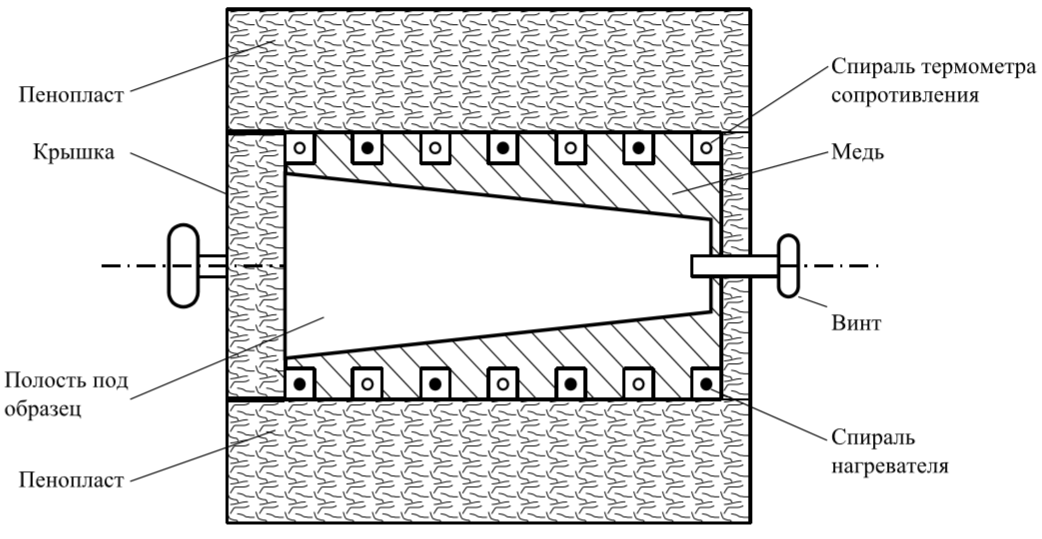
\includegraphics[width=0.8\textwidth]{C:/Users/ПК/Desktop/Учеба/Лабы/Терма/2.1.4/калориметр}
	\caption{Схема устройства калориметра}
	\label{fig:calorimeter}
\end{figure}

Температура измеряется термометром сопротивления, который представляет собой медную проволоку, намотанную на теплопроводящий каркас внутренней стенки калориметра (рис. 1). Сопротивление проводника изменяется с температурой по закону

\begin{equation}
    R_{T} = R_{0}(1 + \alpha \Delta T),
    \label{RT}
\end{equation}

где $R_{T}$ -- сопротивление термеметра про $T  ^{\circ}C$, $R_{0}$ -- его сопротивление при $0  ^{\circ}C$, $\alpha$ -- температурный коэффициент сопротивления. 

Дифференцируя (5) по времени, найдем

\begin{equation}
    \frac{dR}{dt} = R_{0}\alpha \frac{dT}{dt},
    \label{dRT}
\end{equation}

Выразим сопротивление $R_{0}$ через исмеренное значение $R_{\text{к}}$ -- сопротивление термометра при комнатной температуре. Согласно (5), имеем

\begin{equation}
    R_{0} = \frac{R_{\text{к}}}{1 + \alpha \Delta T_{\text{к}}},
    \label{R0}
\end{equation}

Подставляя (6) и (7) в (4), найдем

\begin{equation}
    C = \frac{PR_{\text{к}} \alpha}{(\frac{dR}{dt})_{T_{\text{к}}}(1 + \alpha \Delta T_{\text{к}})},
    \label{capacity}
\end{equation}
 
 Входящий в формулу температурный коэффициент сопротивления меди равен $\alpha = 4,28 \cdot 10^{-3}~\text{град}^{-1}$, все остальные величины определяются экспериментально. 
 
\subsection*{Экспериментальная установка}

Установка состоит из калориметра с пенопластовой изоляцией, помещенного в ящик из многослойной клееной фанеры. Внутренние стенки калориметра выполненым из материала с высокой теплопроводностью. Надежность теплового контакта между телом и стенками обеспечивается их формой: они имеют вид усеченных конусов и плотно прилегают друг к другу. В стенку калориметра вмонтированы электронагреватель и термометр сопротивления. Схема включения нагревателя изображения на рис.2. Система реостатов позволяет установить нужную силу тока в цепи нагревателя. По амперметру и вольтметру определяется мощность, выделяемая в нагревателе. Величина сопротивления термометра измеряется мостом постоянного тока.

\begin{figure}[!h]
	\centering
	\includegraphics[width=0.4\textwidth]{"C:/Users/ПК/Desktop/Учеба/Лабы/Терма/2.1.4/Схема нагревателя"}
	\caption{Схема включения нагревателя}
	\label{fig:boiler}
\end{figure}
 
\section{Ход работы}

Зафиксируем параметры установки и образцов (напряжение и ток в термометре, мощность термометра, массы образцов):

$U = 36~\text{В}, I = 0,3~\text{А}, P = 10,8~\text{Вт}$
\begin{table}[!h]
	\centering
	\begin{tabular}{|l|l|l|}
		\hline
		& Латунный образец & Алюминиевый образец \\ \hline
		Масса, г & $875,5\pm0,1$        & $294,2\pm0,1$           \\ \hline
	\end{tabular}
\end{table}

Также зафиксируем комнатную температуру $T_{\text{к}}$ и сопротивление термометра $R_{\text{к}}$ на момент начала снятия зависимости $R(t)$:

\begin{table}[!h]
	\centering
	\begin{tabular}{|l|l|l|}
		\hline
		& $R_{\text{к}}$, Ом     & $T_{\text{к}}, ^\circ C$    \\ \hline
		Пустой калориметр   & 18,103 & 22,8 \\ \hline
		Латунный образец    & 18,208 & 26   \\ \hline
		Алюминиевый образец & 18,071 & 24,4 \\ \hline
	\end{tabular}
\end{table}

Снимем зависимость $R(t)$ для пустого калориметра и 2 исследуемых образцов, данные занесем в таблицу 1. Перед каждой серией измерений дожидаемся установления комнатной температуры.

\begin{table}[!h]
	\begin{center}
		\scalebox{0.7}{
		\begin{tabular}{|l|l|l|l|l|l|}
			\hline
			\multicolumn{2}{|c|}{Калориметр} & \multicolumn{2}{c|}{Алюминий} & \multicolumn{2}{c|}{Латунь} \\ \hline
			R, Ом           & t, с           & R, Ом         & t, с          & R, Ом        & t, с         \\ \hline
			18,103          & 0              & 18,071        & 0             & 18,208       & 0            \\
			18,153          & 43,56          & 18,121        & 42,45         & 18,258       & 44,97        \\
			18,203          & 87,22          & 18,171        & 99,09         & 18,308       & 89,1         \\
			18,253          & 131,22         & 18,221        & 156,19        & 18,358       & 133,2        \\
			18,303          & 177,59         & 18,271        & 218,49        & 18,408       & 173,33       \\
			18,353          & 225,53         & 18,321        & 282,29        & 18,458       & 243,74       \\
			18,403          & 273,86         & 18,371        & 347,98        & 18,508       & 315,07       \\
			18,453          & 325,84         & 18,421        & 415,6         & 18,558       & 388,62       \\
			18,503          & 378,21         & 18,471        & 485,61        & 18,608       & 466,33       \\
			18,553          & 432,54         & 18,521        & 555,88        & 18,658       & 544,4        \\
			18,603          & 488,09         & 18,571        & 629,67        & 18,708       & 623,27       \\
			18,653          & 544,95         & 18,621        & 702,31        & 18,758       & 704,52       \\
			18,703          & 603,07         & 18,671        & 780,15        & 18,808       & 786,16       \\
			18,753          & 663,26         & 18,721        & 858,52        & 18,858       & 872,43       \\
			18,803          & 724,52         & 18,771        & 937,77        & 18,908       & 959,39       \\
			&                & 18,821        & 1020,88       & 18,958       & 1048,8       \\
			&                &               &               & 19,008       & 1138,5       \\ \hline
		\end{tabular}}
	\end{center}
	\caption{Зависимость сопротивления от времени}
\end{table}

Построим графики зависимости $R(t)$ для полученных данных (Рис. 3).

\begin{figure}[!h]
	\begin{center}
		\subfigure[Пустой калориметр]{\includegraphics[scale=0.4]{"C:/Users/ПК/Desktop/Учеба/Лабы/Терма/2.1.4/Сопротивление от времени калориметр"}}
		\subfigure[Калориметр с алюминиевым образцом]{\includegraphics[scale=0.4]{"C:/Users/ПК/Desktop/Учеба/Лабы/Терма/2.1.4/Сопротивление от времени алюминий"}}
		\subfigure[Калориметр с латунным образцом]{\includegraphics[scale=0.4]{"C:/Users/ПК/Desktop/Учеба/Лабы/Терма/2.1.4/Сопротивление от времени латунь"}}
	\end{center}
	\caption{Зависимость сопротивления термометра от времени}
	\label{fig:графики R(t)}
\end{figure}

Также по полученным данным строим графики зависимостей $\frac{dR}{dT} = f(R)$ (Рис.4) по приближенной формуле $$\frac{dR}{dt}(R)\approx\frac{R(t_{2}) - R(t_{1})}{t_{2} - t_{1}},$$ где $t_{1}$ и $t_{2}$ --- соседние измерения времени, а $R(t_{2}) $ и $ R(t_{1})$ --- значения сопротивления, соответствующие им. Данные, выбивающиеся из тенденции, отбросим.

\begin{figure}[!h]
	\begin{center}
		\subfigure[Пустой калориметр]{\includegraphics[scale=0.35]{"C:/Users/ПК/Desktop/Учеба/Лабы/Терма/2.1.4/dRdt калориметр"}}
		\subfigure[Калориметр с алюминиевым образцом]{\includegraphics[scale=0.35]{"C:/Users/ПК/Desktop/Учеба/Лабы/Терма/2.1.4/dRdt алюминий"}}
		\subfigure[Калориметр с латунным образцом]{\includegraphics[scale=0.35]{"C:/Users/ПК/Desktop/Учеба/Лабы/Терма/2.1.4/dRdt латунь"}}
	\end{center}
	\caption{Зависимость производной $\frac{dR}{dt}$ от сопротивления}
	\label{fig:графики dRdt}
\end{figure}

Экстраполируем полученные зависимости полиномом второй степени до значений $R = R_{\text{к}}$ и вычислим значения $(\frac{dR}{dt})_{T = T_{\text{к}}}$ с использованием полученной формулы.

\begin{table}[!h]
	\centering
	\begin{tabular}{|l|l|l|l|}
		\hline
		& Уравнение экстраполяции                     & $R_{\text{к}}$, Ом     & $(dR/dt)_{R_{\text{к}}}$, Ом/с     \\ \hline
		Калориметр & $y = 0,0002x^2 - 0,0077x + 0,0774$ & 18,103 & 0,003550622 \\ \hline
		Латунь     & $y = 0,0002x^2 - 0,0063x + 0,0626$ & 18,208 & 0,014195853 \\ \hline
		Алюминий   & $y = 0,0004x^2 - 0,0136x + 0,1298$ & 18,071 & 0,014658816 \\ \hline
	\end{tabular}
	\caption{Экстраполяция}
\end{table}

Вычисляем теплоемкость по формуле (8), см. Табл.3.


\begin{table}[!h]
	\begin{center}
		\scalebox{0.85}{
		\begin{tabular}{|l|l|l|l|}
			\hline
			& Теплоемкость, Дж/К & Тепл. без калориметра, Дж/К & Удельная тепл., Дж/кг$\cdot$К \\ \hline
			Калориметр & 214,7216784  & -                            & -                     \\ \hline
			Латунный образец     & 533,5127264  & 318,791048                   & 364,3326263           \\ \hline
			Алюминиевый образец   & 515,9549977  & 301,2333193                  & 1024,603127           \\ \hline
		\end{tabular}}
	\end{center}
	\caption{Результат вычислений теплоемкости}
\end{table}

Все измерения в данной работе проводились мостом и секундомером, поэтому приборные погрешности очень малы; все возможные случайные погрешности несущественны, т.к. относительно измеряемых величин малы также малы. Наиболее существенно на точность исследуемых величин влияет погрешность экстраполяции. При данной выборке она порядка $\varepsilon = 0,1$.

Окончательно, $$c_{\text{латуни}} = 360\pm30 \frac{\text{Дж}}{\text{кг}\cdot\text{К}}$$
$$c_{\text{алюминия}} = 1000\pm100 \frac{\text{Дж}}{\text{кг}\cdot\text{К}}$$

Молярные теплоемкости равны $\mu$c, где с - удельная теплоемкость;
 $\mu_{\text{меди}} \approx 64\frac{\text{г}}{\text{моль}},~ \mu_{\text{цинка}} \approx 65\frac{\text{г}}{\text{моль}},~ \mu_{\text{алюминия}} \approx 27\frac{\text{г}}{\text{моль}}$.

\section{Выводы}

\begin{itemize}
	\item В ходе работы были измерены теплоемкости калориметра, образцов из латуни и алюминия. Были измерены удельные теплоемкости латуни и алюминия: $c_{\text{латуни}} = 360\pm30 \frac{\text{Дж}}{\text{кг}\cdot\text{К}}$,~ $c_{\text{алюминия}} = 1000\pm100 \frac{\text{Дж}}{\text{кг}\cdot\text{К}}$, в пределах погрешности близкие к табличным значениям: $c^{\text{табл.}}_{\text{латуни}} = 380 \frac{\text{Дж}}{\text{кг}\cdot\text{К}}$ и $c^{\text{табл.}}_{\text{алюминия}} = 920 \frac{\text{Дж}}{\text{кг}\cdot\text{К}}$.
	
	
	\item Основной вклад в точность результата внесла погрешность экстраполяции.
	
	\item Экспериментально проверена работоспособность предложенной методики измерения.
\end{itemize}

\end{document}